\documentclass[tikz,border=2mm]{standalone}
\usepackage{pgfplots}
\pgfplotsset{compat=1.18}
\usetikzlibrary{arrows.meta}

\begin{document}
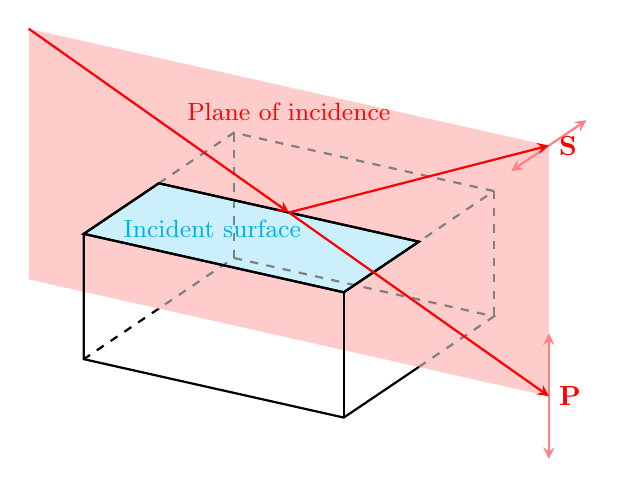
\begin{tikzpicture}
\begin{axis}[
    axis lines=none,          % Completely remove axis lines
    view={120}{25},
    width=12cm,
    height=12cm,
    xmin=-0.5, xmax=1.5,
    ymin=-0.5, ymax=1.5,
    zmin=-0.5, zmax=1.5,
    xtick=\empty,            % Remove x-axis numbers
    ytick=\empty,            % Remove y-axis numbers
    ztick=\empty,            % Remove z-axis numbers
    grid=none,               % Remove grid lines
    plot box ratio=1 1 1,
]

% Define cube vertices
\pgfmathsetmacro{\s}{1} % Cube size
\pgfmathsetmacro{\h}{0.5} % Cube size
\coordinate (O) at (0,0,0);
\coordinate (A) at (\s,0,0);
\coordinate (B) at (\s,\s,0);
\coordinate (C) at (0,\s,0);
\coordinate (D) at (0,0,\h);
\coordinate (E) at (\s,0,\h);
\coordinate (F) at (\s,\s,\h);
\coordinate (G) at (0,\s,\h);

\coordinate (H) at (\h,1.5,0);
\coordinate (I) at (\h,-0.5,0);
\coordinate (J) at (\h,-0.5,1);
\coordinate (K) at (\h,1.5,1);

\coordinate (XhtL) at (0.5,0,0.5);
\coordinate (XhbL) at (0.5,0,0);
\coordinate (XhtR) at (0.5,1,0.5);
\coordinate (XhbR) at (0.5,1,0);

\coordinate (RayS) at (0.5,-0.5,1);
\coordinate (RayM) at (0.5,0.5,\h);
\coordinate (RayE) at (0.5,1.5,1);
\coordinate (RayT) at (0.5,1.5,0);





% Draw cube edges
\draw[thick, dashed, draw=black!50] (O) -- (XhbL);
\draw[thick, dashed, draw=black] (XhbL) -- (A);
\draw[thick, dashed, draw=black!50] (O) -- (C);
\path[fill=red!20] (H) -- (I) -- (J) -- (K) -- cycle; % Plane of incidence
%\draw[thick, fill=cyan!20] (D) -- (E) -- (F) -- (G) -- cycle; % Top face
\draw[thick, fill=cyan!20] (XhtL) -- (E) -- (F) -- (XhtR) -- cycle; % Top face
\draw[thick, dashed, draw=black!50] (XhtL) -- (D) -- (G) -- (XhtR);
\draw[thick, dashed, draw=black!50] (XhbR) -- (C) -- (O) -- (XhbL);

\draw[thick, dashed, draw=black!50] (O) -- (D);
\draw[thick, dashed, draw=black!50] (G) -- (C);
\draw[thick] (XhtL) -- (E) -- (F) -- (XhtR) -- cycle; % Top face

\draw[thick] (XhbR) -- (B) -- (A) -- (E);
\draw[thick] (B) -- (F);



% arrows


\draw[-stealth,thick,red!50] (RayE) -- (0.75,1.5,1) node[right]{};
\draw[-stealth,thick,red!50] (RayE) -- (0.25,1.5,1) node[right]{};


\draw[-stealth,thick,red!50] (RayT) -- (0.5,1.5,0.25) node[right]{};
\draw[-stealth,thick,red!50] (RayT) -- (0.5,1.5,-0.25) node[right]{};


\draw[-stealth,thick,red] (RayS) -- (RayM) node[right]{};
\draw[-stealth,thick,red] (RayM) -- (RayE) node[right]{\textbf{S}};
\draw[-stealth,thick,red] (RayM) -- (RayT) node[right]{\textbf{P}};

\node[text=red] at (0.5,0.5,0.9) {\small{Plane of incidence}};
\node[text=cyan] at (0.75,0.35,0.5) {\small{Incident surface}};



\end{axis}
\end{tikzpicture}
\end{document}